\newpage
\section{Transient Absorption Spectroscopy}
\label{sec:transient}

In this experiment different treatments were investigated in terms of lifetime $\tau$ of the solution itself. At the beginning we expect from theory that the decay of the concentration of the triplet state $C_\mathrm{T}(t)$ is exponential and given by the relation
\begin{gather}
    C_\mathrm{T}(t) = C_\mathrm{T}(0) e^{-k_0 t} + C_\mathrm{T}^\mathrm{Off}~,
    \label{eq:fitExp}
\end{gather}
with the initial concentration $C_\mathrm{T}$ and the decay rate $k_0$. Also, an offset concentration $C_\mathrm{T}^\mathrm{Off}$ was added to encounter any offset cuased by e.g. measuring methods. Since the transient absorption (TA) is porportional to $C_\mathrm{T}(t)$, we can fit the same exponential decay for the transient absorption as well. The full set of fitted treatments and results of the exponential fit can be found in Tab. \ref{tab:lifetimeDecay}. The lifetime $\tau$ was calculated with the relation $\tau = 1/k$. The exponential fits itself are displayed in Fig. \ref{fig:lifetimeDecay}\,.
\begin{center}
    \captionsetup{type = table}
    \begin{tabular}{| c | l | c c |}
        \hline
        No & Treatment             & $k_0$/ms$^{-1}$            & $\tau$/ns   \\\hline
        1  & ZnTPP in BN 0.8\,mM   & 1089 $\pm$ 4               & 919 $\pm$ 3 \\
        2  & ZnTPP in BN 0.6\,mM   & 1077 $\pm$ 5               & 929 $\pm$ 4 \\
        3  & ZnTPP in BN 0.4\,mM   & 1069 $\pm$ 5               & 936 $\pm$ 4 \\
        4  & ZnTPP in BN 0.2\,mM   & 1057 $\pm$ 8               & 946 $\pm$ 7 \\\hline
        8  & ZnTPP in Tol 0.8\,mM  & 1891 $\pm$ 3               & 529 $\pm$ 1 \\\hline
        12 & ZnOEP in BN 0.8\,mM   & 2681 $\pm$ 5               & 373 $\pm$ 1 \\\hline
        \multicolumn{4}{c}{}\\\hline
        No & Treatment             & $k_\mathrm{app}$/ms$^{-1}$ & $\tau$/ns   \\\hline
        5  & ZnTPP:C70 in BN 1:0.1 & 1254 $\pm$ 5               & 798 $\pm$ 3 \\
        6  & ZnTPP:C70 in BN 1:0.2 & 1385 $\pm$ 6               & 722 $\pm$ 3 \\
        7  & ZnTPP:C70 in BN 1:0.3 & 1436 $\pm$ 6               & 697 $\pm$ 3 \\\hline
    \end{tabular}
    \captionof{table}{
        Calculated decay rates $k_0$ and $k_\mathrm{app}$ and lifetimes $\tau$ ($\tau = 1/k$) for different types of treatments.
    }
    \label{tab:lifetimeDecay}
\end{center}

\subsection{Influence of Concentration}
\label{sub:concentration}

First, we want to investigate the influence of concentration on the deacy rate $k_0$, i.e., the lifetime $\tau$. For that we take a closer look at sample number $1-4$ [Tab. \ref{tab:lifetimeDecay}]. In Fig. \ref{fig:lifetimeDecay}\,(a) it is clear that higher maxima correspond with to higher concentration of ZnTPP, which aligns with our expectation that higher concentration leads to a greater amount of absorption. The lifetime $\tau$ on the other hand increases with the reduction of concentration, which follows the expectation from the theory. The kinetics iof the decay of the triplet state are described by the equation
\begin{gather}
    -\frac{\mathrm{d}}{\mathrm{d}t} C_\mathrm{T} = k_1 C_\mathrm{T}(t) + k_2(C_\mathrm{T}(t))^2 + k_3C_\mathrm{T}(t)C_\mathrm{G}(t)~,
    \label{eq:kineticsTriplet}
\end{gather}
where $C_\mathrm{G}(t)$ is the concentration of the ground state and $k_1, k_2, k_3$ are decay rates. In further calculation the assumption $C_\mathrm{T}(t) \ll C_\mathrm{G}(t)$ will be made, which leads to the discussed exponential decay [Eq. (\ref{eq:fitExp}), Chapter \ref{sec:decay}]. But, this assumption gets less valid for an increasing population of triplet states, to the point at which one has to take the terms with $C_\mathrm{T}(t)$ into account. This results in higher decay rates $k_0$ and shorter lifetimes $\tau$ of the triplet states. The same behaviour can be identife to the cases of higher concentration of ZnTPP in BN and explains the kinetics of the decay process.

\subsection{Influence of Fullerene \boldmath{$\mathrm{C}_{70}$}}
\label{sub:fullerene}

In the next paragraph the impact of the fullerene $\mathrm{C}_{70}$ on the lifetime $\tau$ will be addressed. We consider for this analysis sample 1 (base solution) and $5-7$ [Tab. \ref{tab:lifetimeDecay}]. In Fig. \ref{fig:lifetimeDecay}\,(b) one can see that the decreases the higher the concentration of the fullerene $C_\mathrm{q}$ gets, introducing a quenching process. This result was expected, because in theory the decay rate $k_0$ gets expanded as
\begin{gather}
    k_0 \longrightarrow k_\mathrm{app} = k_0 + k_\mathrm{q}C_\mathrm{q}~,
    \label{eq:decayExpand}
\end{gather}
with the new decay rate $k_\mathrm{app}$ and the reaction rate of quenching process $k_\mathrm{q}$. The expansion of the decay rate $k_0$ leads to higher decay rates $k_\mathrm{app}$ ($k_\mathrm{q} > 0$), which leads to shorter lifetimes $\tau$. To determine the quenchning reaction rate $k_\mathrm{q}$, we take the calculated decay rates $k_\mathrm{app}$ and fit them against the concentration $C_\mathrm{q}$ [Eq. \ref{eq:decayExpand}]. For the decay rate $k_0$ the decay rate of the base solution (sample 1) will be used. From the slope of the linear fit one can calculate the quenchning reaction rate $k_\mathrm{q}$. The linear fit can be seen in Fig. \ref{fig:concentration}. 

\begin{center}
    \captionsetup{type = figure}
    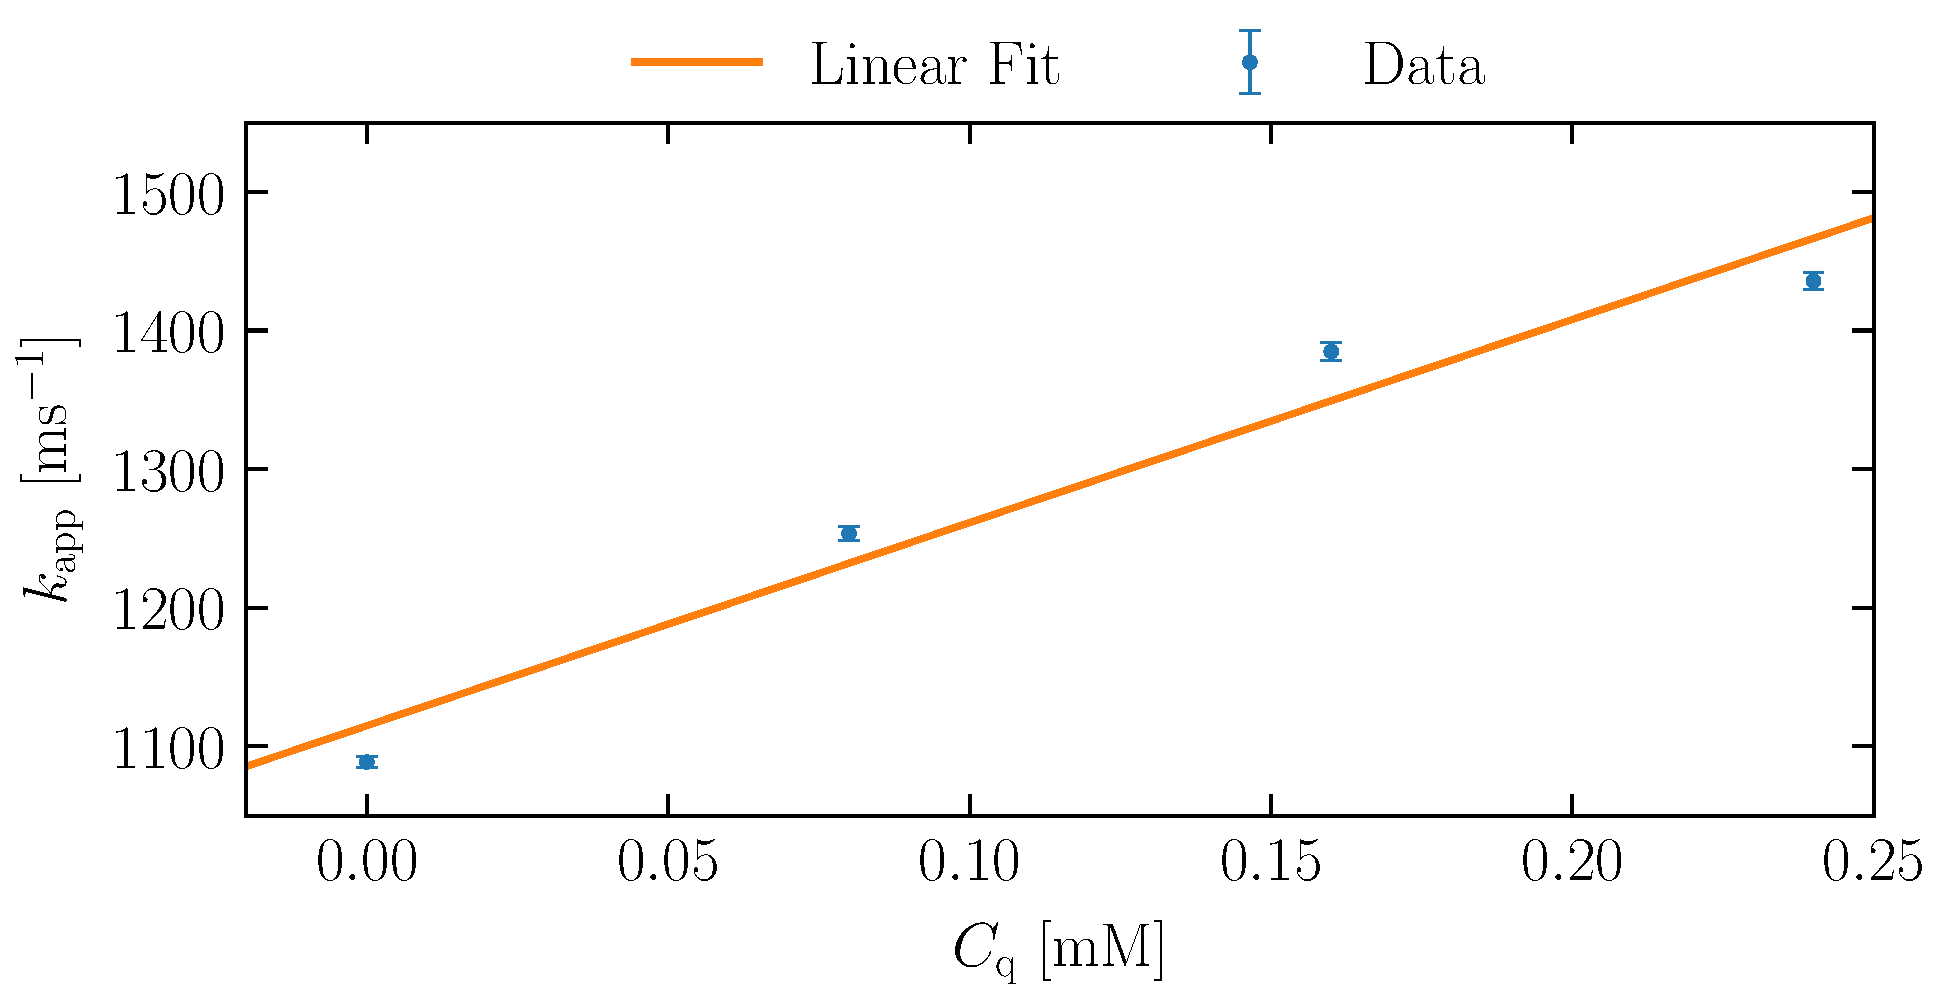
\includegraphics[width = 0.85\textwidth]{Pictures/Evaluation/42/Concentration.pdf}
    \captionof{figure}{
        Linear fit of decay rate $k_\mathrm{app}$ for different fullerene concentration $C_\mathrm{q}$. 
    }
    \label{fig:concentration}
\end{center}

The calculation yields
\begin{gather*}
    \boxed{k_\mathrm{q} = (1.5 \pm 0.2) \times 10^9\,\mathrm{sM^{-1}}}~, %1465.49 229.41 ms-1/mM
\end{gather*}
which does not align with the result of Ito et al.\cite{Nojiri.1998}, who determined $k_\mathrm{q} = 4.7 \times 10^9\,\mathrm{sM^{-1}}$, but is in the right order of magnitude.

\subsection{Influence of the Solvent}
\label{sub:difference}

In this paragraph the influence of Solvent on the transient absorption (TA) signal and the lifetime $\tau$ will be dicussed. 
\bigskip

First, we look at the variation of ZnTPP with BN and Tol for the concentration 0.8\,mM (sample 1 and 8 [Tab. \ref{tab:lifetimeDecay}]). In Fig. \ref{fig:lifetimeDecay}\,(c) we can observe the nearly same maximum value for both solutions but different lifetimes $\tau$, which are calculated in Tab. \ref{tab:lifetimeDecay}. This aligns with the UV-VIS spectroscopy from Chapter \ref{sec:uv-vis}, because the polarity of BN makes it easier to induce more charges into the delocalized $\pi$-electron system. So, it is possible to observe a redshift and an increase of lifetime $\tau$. 
\bigskip

Next, we vary the zinc complexes of the solution from ZnTPP to ZnOEP, but we keep BN as second solvent of the solution with concentration 0.8\,mM (sample 1 and 12 [Tab. \ref{tab:lifetimeDecay}]). The transient absorption signal can be found in Fig. \ref{fig:lifetimeDecay}\,(d) with the corresponding decay rates $k$ and lifetimes $\tau $ in Tab. \ref{tab:lifetimeDecay}. It is clearly visible that the maximum of the TA signal is for both zinc complexes the same but the lifetime $\tau$ for is much shorter for ZnOEP. The value of the TA maximum corresponds with the maximum concentration of the triplet state and is therefor correlated to the absorption of the pump laser light. Looking at the UV-VIS of ZnTPP and ZnOEP [Fig. \ref{fig:uv-visZinc}] one can conclude that the absorbance for ZnTPP and ZnOEP does not differ from each other, which explains teh same maximum value for the TA signal. The longer lifetime $\tau$ of ZnTPP can also be linked to the redshift compared to ZnOEP. Due to the four additional phenyl groups in ZnTPP, the conjugated electron system is bigger than in ZnOEP. So, a lower energy is needed to exite the electrons of ZnTPP.
\bigskip

Finally, we want to discuss the variation of the solution itself. For that, we take a look at sample 1 (ZnTPP in BN 0.8\,mM) and 9 (P3HT in Tol 1.5\,mM). In Fig. \ref{fig:difference} it is visible that P3HT has a smaller maximum compared to ZnTPP. From the previous lifetime analysis one can assume trivial that the lifetime of P3HT is shorter compared to the lifetime of ZnTPP. Comparing the UV-VIS of P3HT from Ref. \citenum{Rahimi2014} to the evaluation from ZnTPP from Chapter \ref{sec:uv-vis} the observed redshift is also present for P3HT as well as the smaller absorbance compared to ZnTPP. The underlying process relates to the P3HT aggregates, which can consist of crystalline regions, amorphous domains or a combination of both. Amorphous chain sequences lead to structural defects, grain boundaries and coiled-like chain conformations that can reduce intra-chain order. Therefore, UV-VIS absorption signatures are broadened and blue shifted towards higher energies \cite{Rahimi2014}, which results in the observed (TA) signal.

\begin{center}
    \captionsetup{type = figure}
    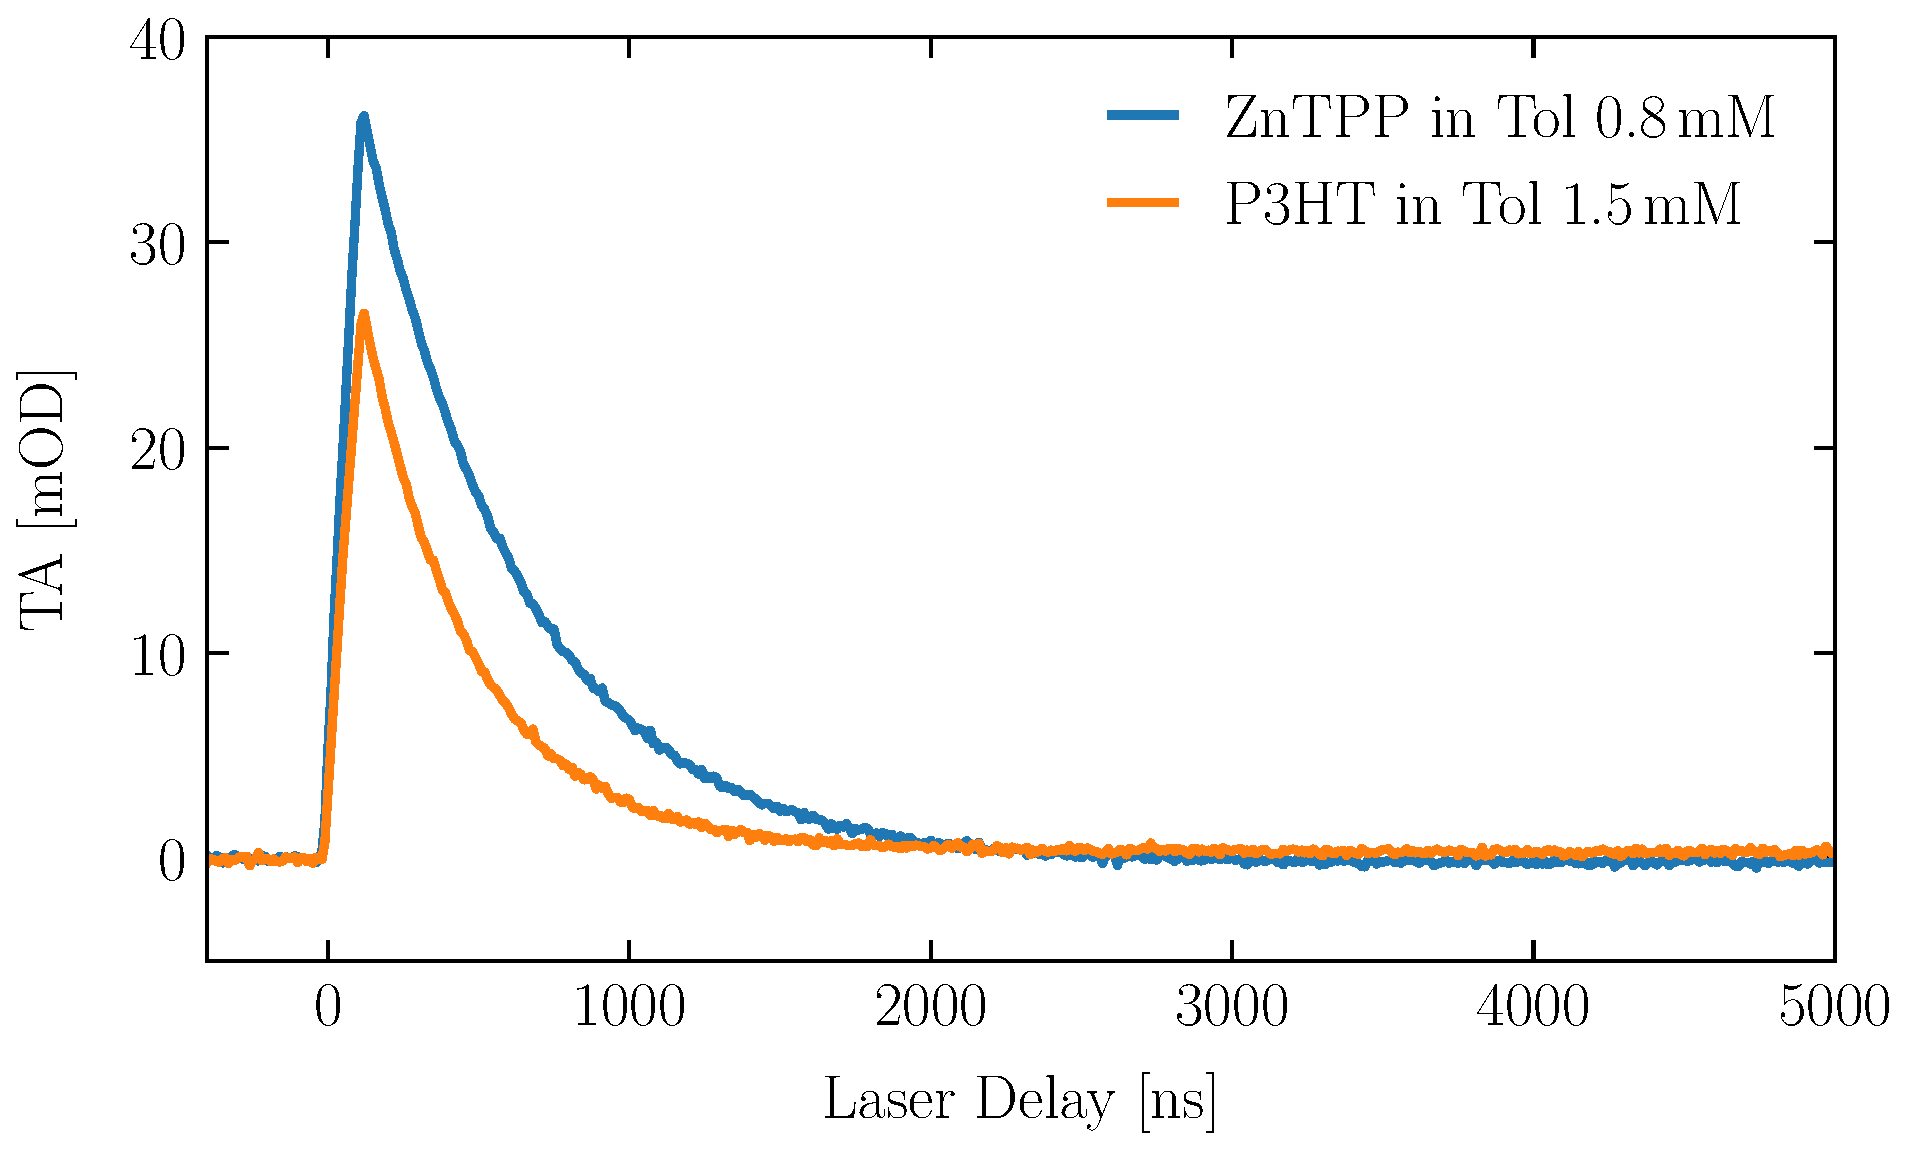
\includegraphics[width = 0.85\textwidth]{Pictures/Evaluation/42/Difference.pdf}
    \captionof{figure}{
        Transient absorption signal using different treatments with ZnTPP and P3HT 
    }
    \label{fig:difference}
\end{center}

\begin{center}
    \begin{sidewaysfigure}
    \centering
    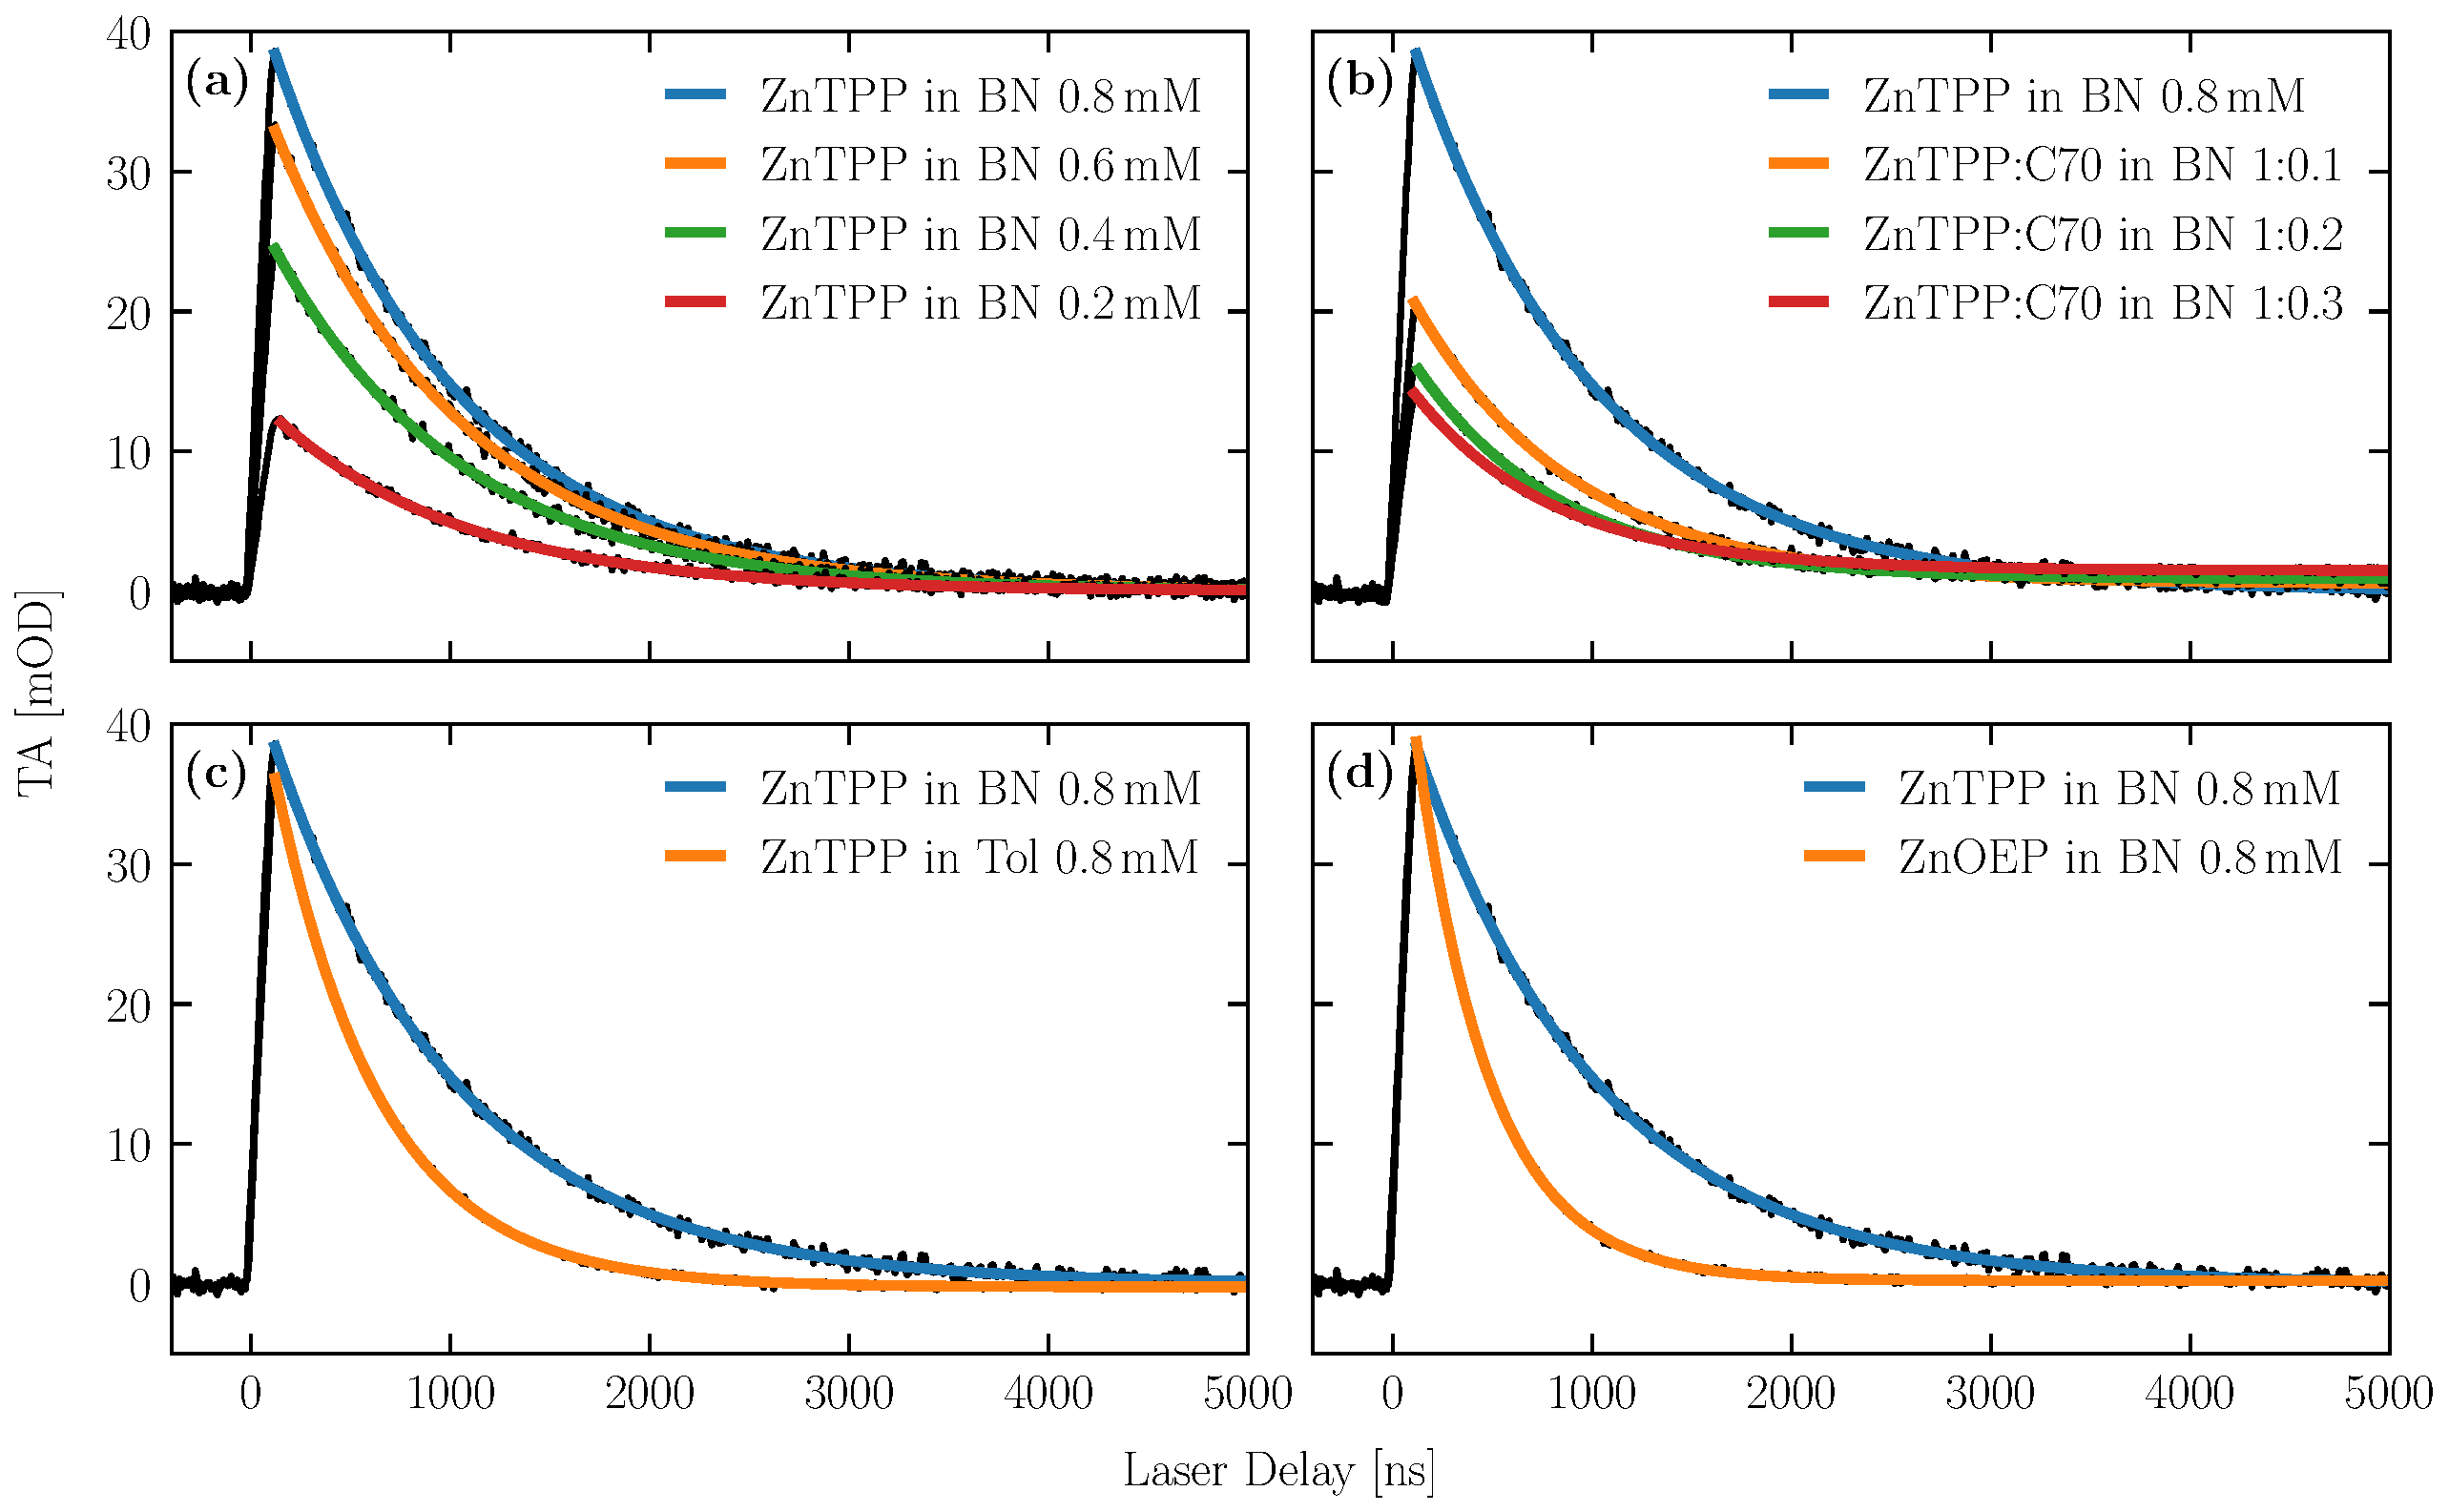
\includegraphics[width = 0.9\textheight]{Pictures/Evaluation/42/Lifetime.pdf}
    \caption{
        Comparison between data of the transient absorption of different treatments with the exponential fits colored for each treatment: (a) Different concentration of ZnTPP in BN, (b) Different dullutions of C$_{70}$ in ZnTPP in BN 0.8\,mnM, (c) Different Solvents (BN, Tol) with ZnTPP and a concentration of 0.8\,mM and (d) Different Solvents (ZnTPP, ZnOEP) with BN and a concentration of 0.8\,mM.
    }
    \label{fig:lifetimeDecay}
    \end{sidewaysfigure}
\end{center}
\newpage

\subsection{Influence of the Pump Laser Width}
\label{sub:pumpLaser}

\begin{center}
    \captionsetup{type = figure}
    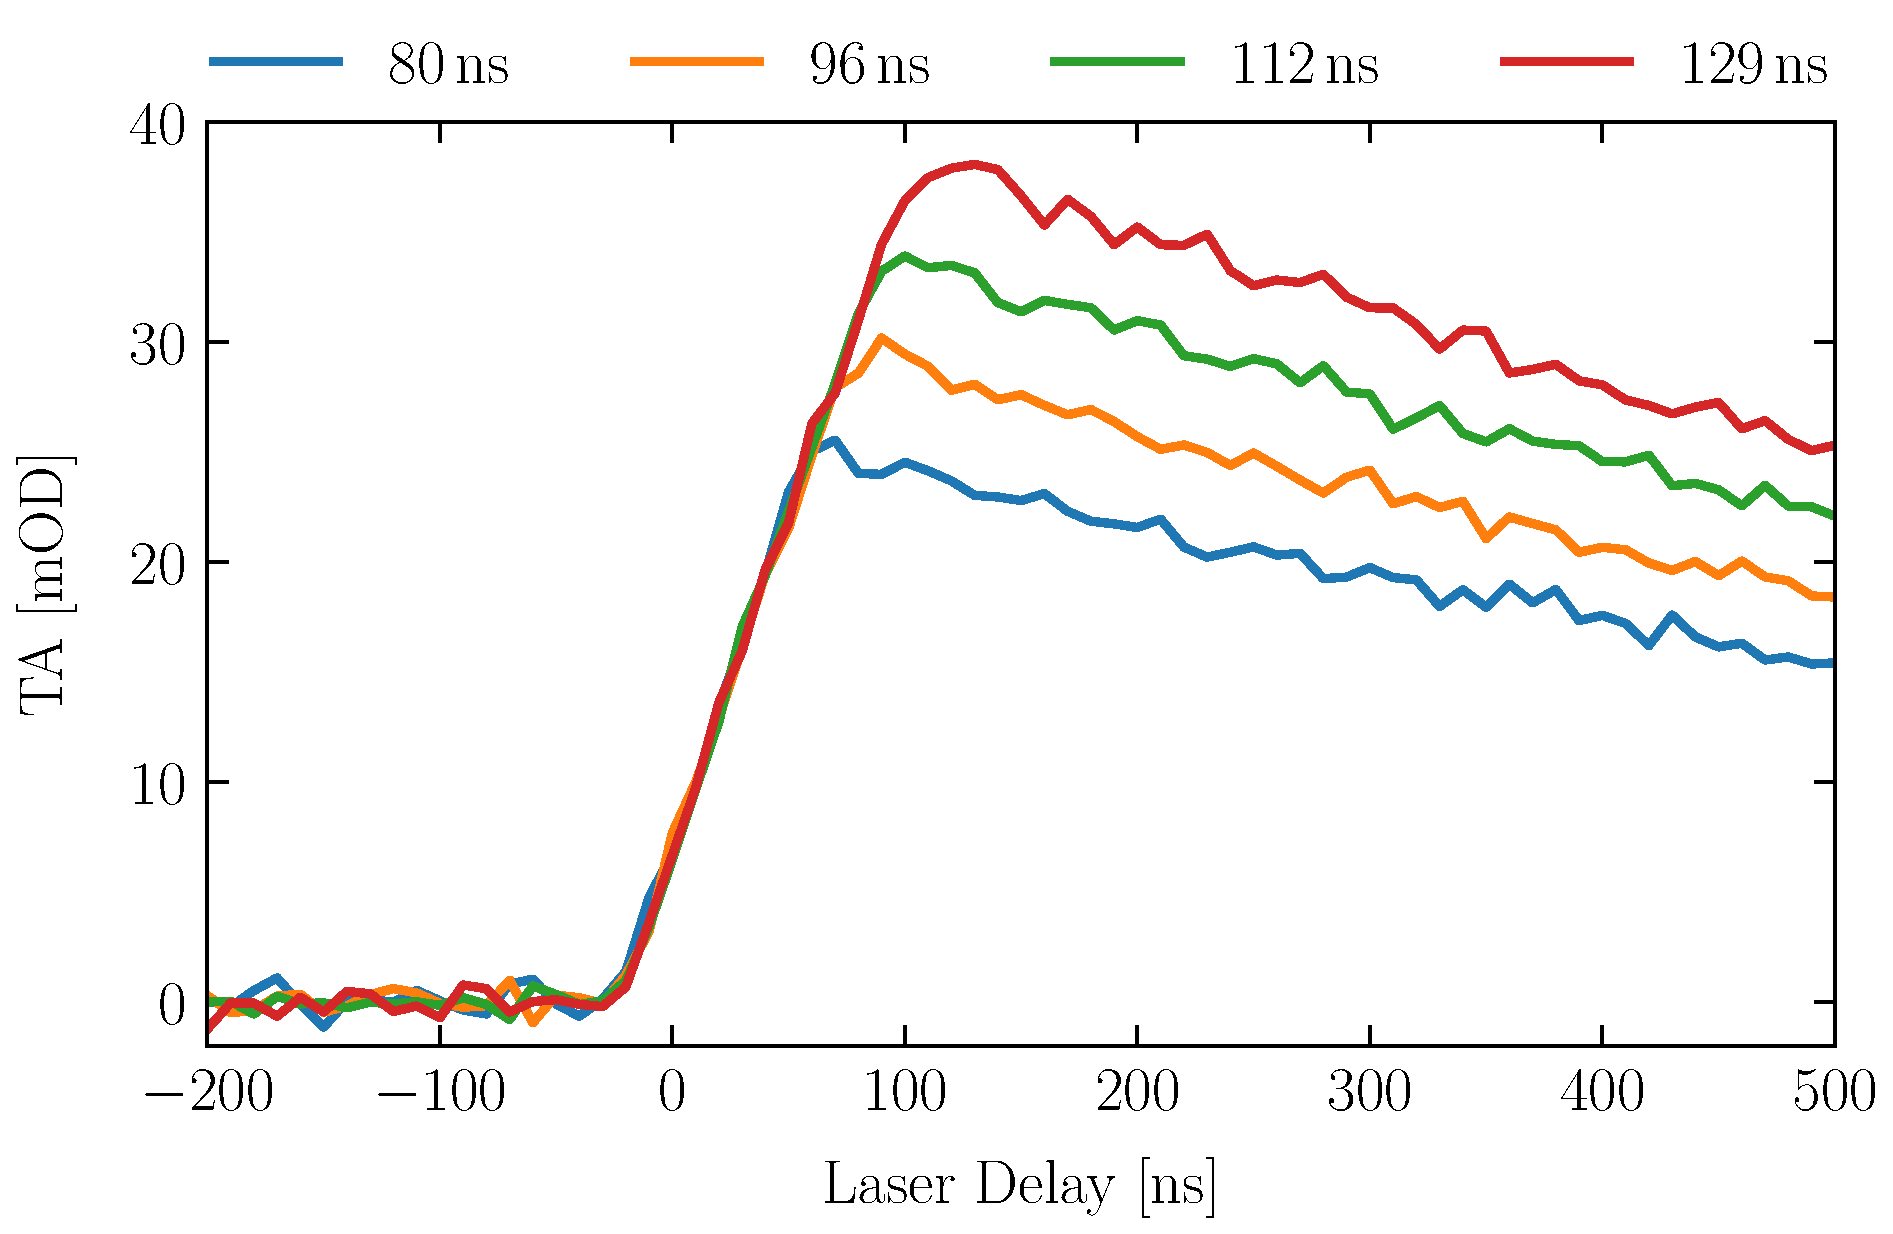
\includegraphics[width = 0.85\textwidth]{Pictures/Evaluation/42/Pump-Laser.pdf}
    \captionof{figure}{
        Transient absorption signal for different pump laser widths using ZnTPP in BN 0.8\,mM.
    }
    \label{fig:pumpLaser}
\end{center}

To investigate the influence of the pump laser width on the transient absorption (TA) signal, we measured for sample 1 [Tab. \ref{tab:lifetimeDecay}] the TA using four different pump laser widths. The TA signal is displayed in Fig. \ref{fig:pumpLaser}. In Fig. \ref{fig:pumpLaser} one can see that there is a shift in the TA maxima which correspond with the set pump laser width. This follows our expectations, since the longer pump laser should be able to exite more electrons to the triplet state. A closer look also shows that the pump laser width has no influnce on the decay rate $k_0$, i.e., the lifetime $\tau$. But to be sure a longer time interval has to be measured to determine the long time behaviour of the decay process.